\documentclass[border=10pt]{standalone}

\usepackage{tikz}
\usepackage{tikzsymbols}
\usetikzlibrary{calc,patterns,shapes.geometric}

\def\centerarc[#1](#2)(#3:#4:#5){\draw[#1] ($(#2)+({#5*cos(#3)},{#5*sin(#3)})$) arc (#3:#4:#5);}

\begin{document}
	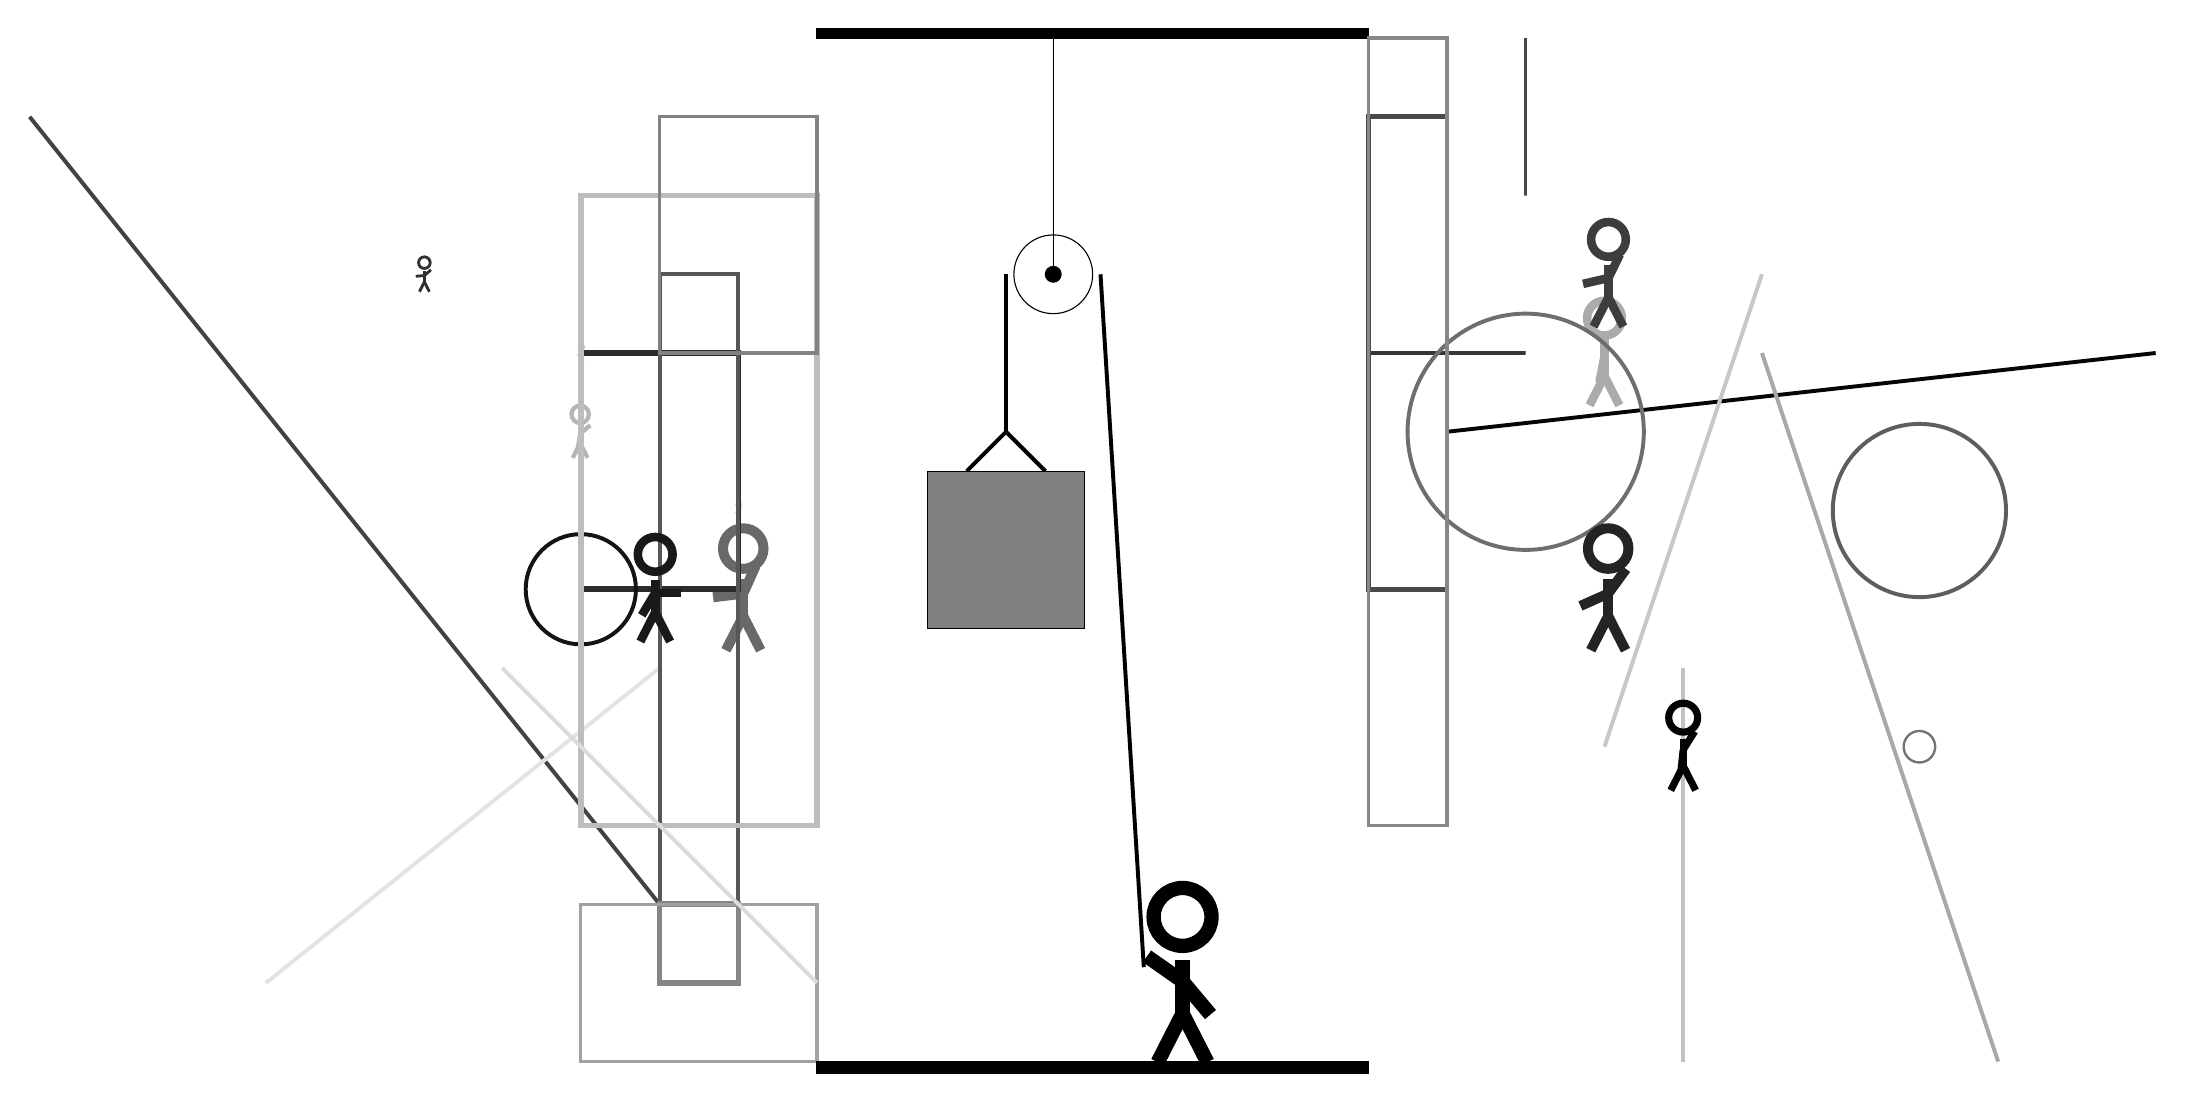
\begin{tikzpicture}
		%%%%% START %%%%%
		
		\draw[fill=black] (-2, 10) rectangle (5, 10.125);
		
		\draw (1, 7) circle (0.5);
		\draw[fill=black] (1, 7) circle (0.1);
		\draw (1, 10) -- (1, 7);
		
		\draw [line width=0.5mm, color=black!63](12, 4) circle (1.1);
		
		\draw[line width=0.5mm, color=black!74](-4, -1) -- (-12, 9);
		\draw [line width=0.6mm, color=black!48](-9, 3) circle (0.0);
		\node[line width=0.6mm, color=black!33] at (8, 6) {\Strichmaxerl[6][79][90]};
		\draw[line width=0.4mm, color=black!72] (7, 10) rectangle (7, 8);
		
		\draw[line width=0.5mm, color=black!24](9, -3) -- (9, 2);
		\draw[line width=0.5mm, color=black!98](6, 5) -- (15, 6);
		
		\node[line width=0.4mm, color=black!59] at (-3, 3) {\Strichmaxerl[7][7][66]};
		\node[line width=0.2mm, color=black!29] at (-5, 5) {\Strichmaxerl[3][81][40]};
		
		\node[line width=0.6mm, color=black!24] at (-5, 6) {\Strichmaxerl[1][19][83]};
		
		\draw[line width=0.5mm, color=black!79] (5, 6) rectangle (7, 6);
		\draw [line width=0.3mm, color=black!55](12, 1) circle (0.2);
		\draw[line width=0.5mm, color=black!34] (-2, 4) rectangle (-2, 2);
		
		\node[line width=0.6mm, color=black!13] at (-3, 4) {\Strichmaxerl[1][25][45]};
		\node[line width=0.4mm, color=black!76] at (8, 7) {\Strichmaxerl[6][13][64]};
		\draw [line width=0.5mm, color=black!57](7, 5) circle (1.5);
		
		\draw[line width=0.7mm, color=black!83] (-3, 3) rectangle (-5, 6);
		\draw[line width=0.5mm, color=black!22](10, 7) -- (8, 1);
		\draw[line width=0.5mm, color=black!11](-4, 2) -- (-9, -2);
		\node[line width=0.4mm, color=black!86] at (8, 3) {\Strichmaxerl[7][24][54]};
		\node[line width=0.7mm, color=black!99] at (9, 1) {\Strichmaxerl[5][84][58]};
		
		\draw[line width=0.5mm, color=black!66] (-3, -1) rectangle (-4, 7);
		
		\draw[line width=0.6mm, color=black!71] (5, 9) rectangle (6, 3);
		\draw [line width=0.5mm, color=black!92](-5, 3) circle (0.7);
		\draw[line width=0.5mm, color=black!34](10, 6) -- (13, -3);
		\draw[line width=0.7mm, color=black!48] (-3, -1) rectangle (-4, -2);
		
		\node[line width=0.6mm, color=black!90] at (-4, 3) {\Strichmaxerl[6][59][0]};
		\draw[line width=0.4mm, color=black!47] (5, 0) rectangle (6, 10);
		\draw[line width=0.7mm, color=black!26] (-2, 0) rectangle (-5, 8);
		\draw[line width=0.4mm, color=black!49] (-2, 6) rectangle (-4, 9);
		\draw[line width=0.4mm, color=black!37] (-2, -1) rectangle (-5, -3);
		\node[line width=0.5mm, color=black!81] at (-7, 7) {\Strichmaxerl[2][5][41]};
		\draw[line width=0.5mm, color=black!14](-6, 2) -- (-2, -2);
		
		
		\draw[line width=0.5mm] (-0.1, 4.5) -- (0.4, 5.0) -- (0.9, 4.5);
		\draw[fill=black!50] (-0.6, 4.5) rectangle (1.4, 2.5);
		
		\draw[line width=0.5mm] (0.4, 7) -- (0.4, 5.0);
		\centerarc[line width=0.5mm](1, 7)(0:180:0.6);
		\draw[line width=0.5mm](1.6, 7) -- (2.15, -1.8);
		
		\node at (2.6, -1.9) {\Strichmaxerl[10][-35][-50]};
		
		\draw[fill=black] (-2, -3) rectangle (5, -3.15);
		
		%%%%% END %%%%%
	\end{tikzpicture}
\end{document}